\glsresetall
\chapter{Methodology}
\label{chap:methodology}

The methodology of work carried out in this research project is presented in this chapter. First, every member involved will be mentioned as well as their individual contribution for the project. Second, the adopted approach and organisation process of the collaborators involved will be explained. Finally, the work plan including foreseen and real work plans for the whole year are presented and discussed.

The main people involved in this project were myself, André Pascoal Bento, student at the Master course of Informatics Engineering at \gls{dei}, who carried out the investigation and development of the project. In second, Prof. Filipe Araújo, assistant professor at the University of Coimbra, who contributed with his vast knowledge and guidance on topics about distributed systems and cloud computing. In third, Prof. Jorge Cardoso, Chief Architect for Intelligent CloudOps at Huawei Technologies, who contributed with his vision, great contact with the topics addressed in this work and with the tracing data set from Huawei Cloud Platform~\cite{huawei_cloud_platform}. In fourth, Eng. Jaime Correia, doctoral student at \gls{dei}, who contributed with his vast technical knowledge regarding the topics of tracing and monitoring microservices. In Sixth, Eng. Ricardo Filipe, doctoral student at \gls{dei}, who contributed with peer review of the paper produced for the International Symposium on Network Computing and Applications (IEEE NCA 2019).
% , like the ones mentioned before,

This work stands for an investigation and was mainly an exploratory work, therefore, no development methodology was adopted. Meetings were scheduled to happen every two weeks. In these meetings, every participant element in the project joined with the objective of discussing the work carried out in the last two weeks and define the new course of research. In the first semester, topics like published papers, state of the art, analysis of related work and a proposition of solution were the main focus. In the second semester, two more colleagues joined the whole project (DataScience4NP). One of them with a project somehow related to this research. They started participating in meetings and this contributed with a wider discussion of ideas. In these meeting, the main topics covered were: implementation of the proposed solution, research for algorithms and methods for trace processing and analysis of gathered data. In the end, these meetings were more than enough to keep the productivity and good work.

Total time spent in each semester, by week, were sixteen $(16)$ hours for the first semester and forty $(40)$ hours for the second. In the end, it was spent a total of three-hundred and four $(304)$ hours for the first semester, starting in $11.09.2018$ and ending in $21.01.2019$ $(19$ weeks $*$ $16$ hours per week$)$. For the second semester, eight-hundred and forty $(840)$ hours were spent, starting in $04.02.2019$ and ending in $28.06.2019$ $(21$ weeks $*$ $40$ hours per week$)$.

Before starting this research project, there was a work plan defined for two semesters presented in the proposition. For purposes of analysis and comparison, these plans, proposed and real of both semesters, are presented in Figures~\ref{fig:proposed_work_plan_semester_1_and_2} and~\ref{fig:real_work_plan_semester_1}.

As we can see in Figures~\ref{fig:proposed_work_plan_semester_1_and_2} and~\ref{fig:real_work_plan_semester_1}, the proposed work for the first semester has suffered some changes, when comparing it to the real work plan. Task 1 - Study the state of the art(...), was branched in two, 1 - Project Contextualisation and Background and 2 - State of the Art, however, these last ones tocked more time to accomplish due to lack of work in the field of trace processing and trace analysis, core topics for this thesis. Task 2 - Integrate the existing work was replaced by task 3 - Prototyping and Technologies Hands-On due to redirections in the work course. This redirection was done due to interest increase in testing state of the art technologies, allowing us to get a better visualisation of the data provided by Huawei and enhancing our investigation work. The remaining tasks took almost the predicted time to accomplish.

For the second semester, an ``expected'' work plan was defined with respect to the proposed work, presented in Figure~\ref{fig:proposed_work_plan_semester_1_and_2}, and the state of the research at the time. The expected work plan can be visualized in Figure~\ref{fig:complete_work_plan_semester_2}. This Figure contains the expected (Grey) and real (Blue) work for the second semester.

%To estimate the effort for each task, we decided to: First, group tasks in four groups depending on complexity and work load. Second, discuss if they were in the right group taking into consideration what is defined in the solution and the task background knowledge. Third, assign the defined values to each group. This values represent the work days for each task, and in this case we defined the following four: 3(three), 5(five), 8(eight) and 12(twelve) working days as they are akin to the Fibonacci suites~\cite{project_estimation_times}. The only task that were not submitted to this, was the task 3 - Write the final report.

Three main changes were made over time in the work plan. The first one involved a reduction in task 1 - Metrics collector tool. When the solution was being implemented and the prototype was capable to extract a set of metrics, we decided to stop the implementation process to analyse the research questions. Second, this analysis lead to an emergence of ideas, ``2 - Restructuring research questions',' and thus a project redirection. Tests were removed from planning and the project followed with the objective of producing the data analyser, ``3 - Data Analyser tool'', and with it, answer two main questions regarding anomalous services and quality of tracing. Third, the introduction of a new task, ``4 - Write paper to NCA 2019'', covering the work presented in this thesis.

These Figures have been created by an open-source tool called GanttProject~\cite{gantt_project_tool} that produce Gantt charts, a kind of diagram used to illustrate the progress of the different stages of a project.

Next, Chapter~\ref{chap:state_of_the_art}~-~\nameref{chap:state_of_the_art}, the state of the field is covered with core concepts, technologies and related work.

\begin{landscape}
    \begin{figure}
        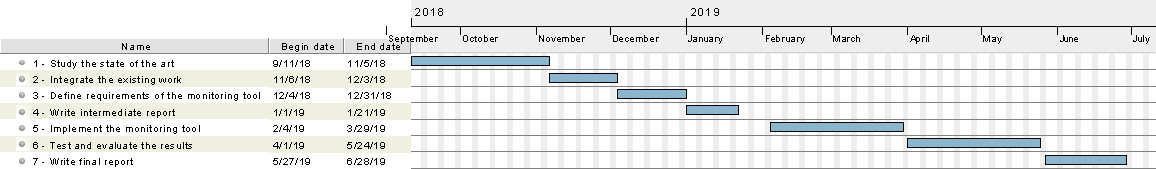
\includegraphics[height=0.234\textwidth]{images/proposed_work_plan_semester_1_and_2.pdf}
        \caption{Proposed work plan for first and second semesters.}
        \label{fig:proposed_work_plan_semester_1_and_2}
        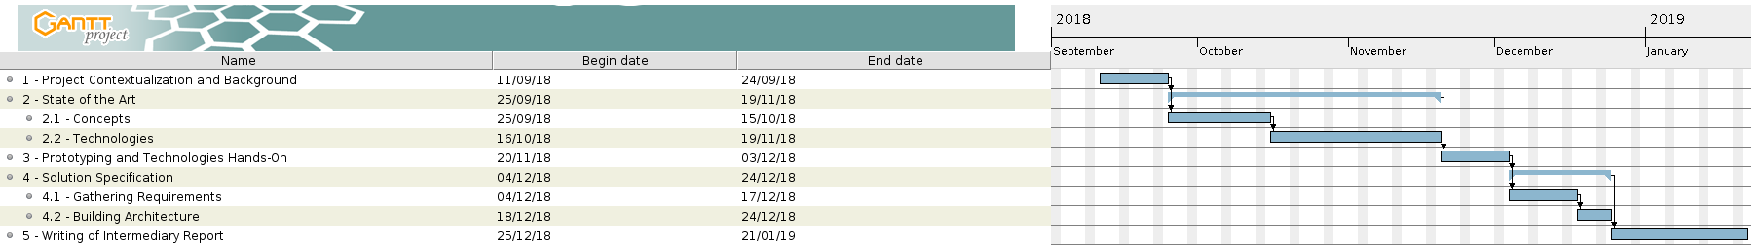
\includegraphics[height=0.3\textwidth]{images/real_work_plan_semester_1.pdf}
        \caption{Real work plan for first semester.}
        \label{fig:real_work_plan_semester_1}
    \end{figure}
\end{landscape}

\begin{landscape}
    \begin{figure}
        %\includegraphics[width=1.0\textwidth]{Image.eps}
        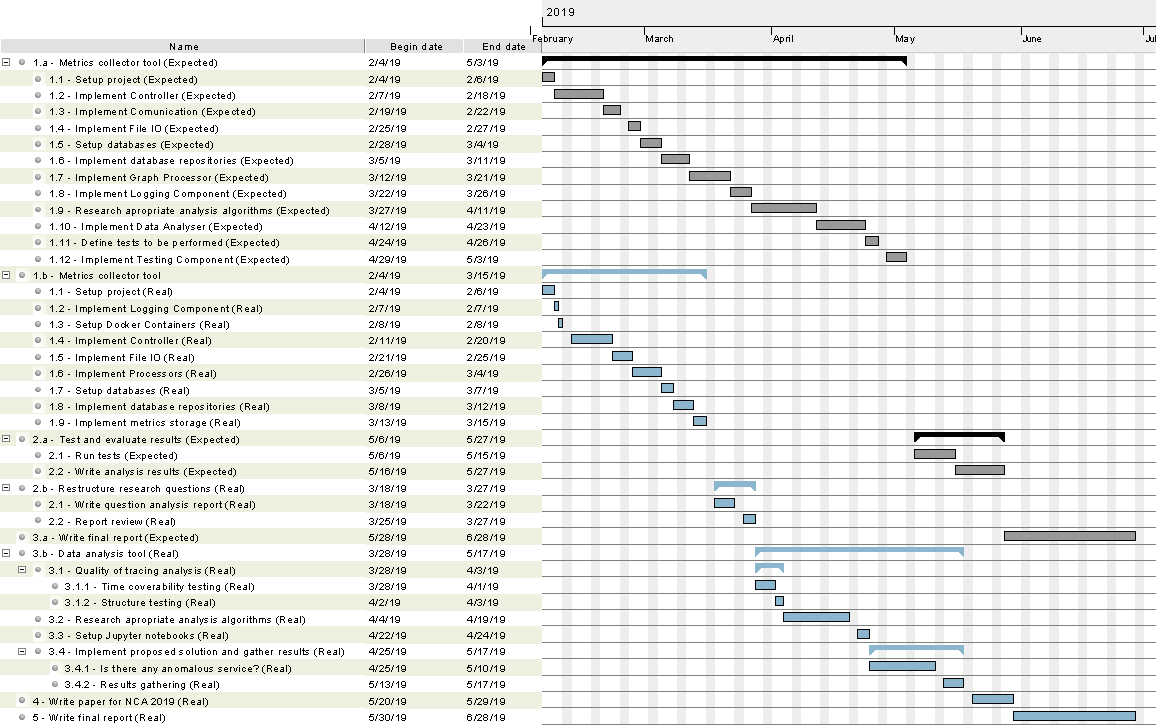
\includegraphics[height=1.0\textheight]{images/complete_work_plan_semester_2.pdf}
        \caption{Real and expected work plans for second semester.}
        \label{fig:complete_work_plan_semester_2}
    \end{figure}
\end{landscape}

\checkoddpage
\ifthenelse{\boolean{oddpage}}
{ % Odd page
    \newpage
    \blankpage}
{ % Even page
}